\begin{pastexam}[label={px:ccu-115-swa-09}]{中正資工所甲組 115 學年度 第 19 題}
（複選；全對才給分）

(2\%) (\qquad) Based on the results of the previous two questions and the given graph, identify the
articulation points.

（前兩題：For determining the articulation points in the following graph, list the depth-first search
numbers (starting from 1) for each vertex in the order of $A, B, C, D, E, F, G, H,$ and $I$. Begin
the depth-first search at \textbf{vertex $A$}. If multiple unvisited vertices are available during
the search, select the vertex with the smallest alphabetical label. 接著求每個頂點的 $low(v)$。）
\begin{center}
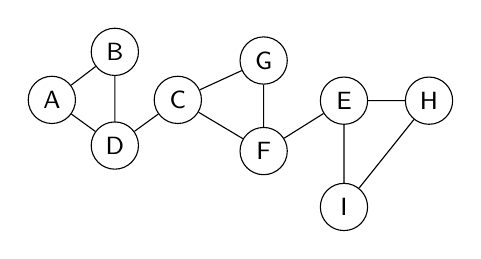
\begin{tikzpicture}[x=1cm,y=1cm,v/.style={circle,draw,minimum size=6mm,inner sep=1pt,font=\small\sffamily}]
\node[v] (A) at (0.75,-1.17) {A};
\node[v] (B) at (1.55,-0.56) {B};
\node[v] (D) at (1.55,-1.75) {D};
\node[v] (C) at (2.35,-1.17) {C};
\node[v] (G) at (3.44,-0.67) {G};
\node[v] (F) at (3.44,-1.82) {F};
\node[v] (E) at (4.46,-1.18) {E};
\node[v] (H) at (5.54,-1.18) {H};
\node[v] (I) at (4.46,-2.53) {I};
\draw (A)--(B) (A)--(D) (B)--(D) (D)--(C) (C)--(G) (C)--(F) (G)--(F) (F)--(E) (E)--(H) (E)--(I) (H)--(I);
\end{tikzpicture}
\end{center}
(a)~(A, C, E, I) \qquad (b)~(B, G, E) \qquad (c)~(C, D, E, F) \qquad (d)~(A, C, E)\\
(e)~none of the above
\end{pastexam}

\begin{pastsoln}
答案：(c)。

用前兩題（歷屆試題~\ref{px:ccu-115-swa-07}、\ref{px:ccu-115-swa-08}）的 $d$ 和 $\mathit{low}$，套資結書
第~23.5~節的兩個判斷（資結書定理~23.8、23.9）：
\begin{itemize}
\item 根 A：是割點若且唯若它在 DFS 樹上有兩個以上子節點。 A 只有一個子節點 B，不是割點。
\item 非根的 $u$：是割點若且唯若有某個子節點 $v$ 滿足 $\mathit{low}[v] \ge d[u]$。
\end{itemize}
\begin{center}
\small
\begin{tabular}{ccccl}
\toprule
$u$ & $d[u]$ & 子節點 $v$ & $\mathit{low}[v]$ & 判斷 \\
\midrule
B & 2 & D & 1 & $1 < 2$，不是 \\
D & 3 & C & 4 & $4 \ge 3$，\textbf{割點} \\
C & 4 & F & 4 & $4 \ge 4$，\textbf{割點} \\
F & 5 & E, G & 6, 4 & E 那邊 $6 \ge 5$，\textbf{割點} \\
E & 6 & H & 6 & $6 \ge 6$，\textbf{割點} \\
H & 7 & I & 6 & $6 < 7$，不是 \\
G, I & & — & & 葉節點，不是 \\
\bottomrule
\end{tabular}
\end{center}
割點是 C、D、E、F，就是 (c)。 直接看圖也對得上：拿掉 D，A、B 和其他分開；拿掉 C，A--B--D 和
F--G 那邊分開；拿掉 F，E--H--I 和 C--G 那邊分開；拿掉 E，H--I 和其他分開。
\begin{itemize}
\item (a) 錯：A 是只有一個子節點的根；I 是葉節點。
\item (b) 錯：B 拿掉後 A--D 仍相連；G 拿掉後 C--F 仍相連。
\item (d) 錯：A 不是，而且漏了 D、F。
\item (e) 錯，(c) 對。
\end{itemize}
\end{pastsoln}
